%%
%% This is file `sample-sigconf-authordraft.tex',
%% generated with the docstrip utility.
%%
%% The original source files were:
%%
%% samples.dtx  (with options: `all,proceedings,bibtex,authordraft')
%% 
%% IMPORTANT NOTICE:
%% 
%% For the copyright see the source file.
%% 
%% Any modified versions of this file must be renamed
%% with new filenames distinct from sample-sigconf-authordraft.tex.
%% 
%% For distribution of the original source see the terms
%% for copying and modification in the file samples.dtx.
%% 
%% This generated file may be distributed as long as the
%% original source files, as listed above, are part of the
%% same distribution. (The sources need not necessarily be
%% in the same archive or directory.)
%%
%%
%% Commands for TeXCount
%TC:macro \cite [option:text,text]
%TC:macro \citep [option:text,text]
%TC:macro \citet [option:text,text]
%TC:envir table 0 1
%TC:envir table* 0 1
%TC:envir tabular [ignore] word
%TC:envir displaymath 0 word
%TC:envir math 0 word
%TC:envir comment 0 0
%%
%% The first command in your LaTeX source must be the \documentclass
%% command.
%%
%% For submission and review of your manuscript please change the
%% command to \documentclass[manuscript, screen, review]{acmart}.
%%
%% When submitting camera ready or to TAPS, please change the command
%% to \documentclass[sigconf]{acmart} or whichever template is required
%% for your publication.
%%
%%
\documentclass[sigconf, screen, review, anonymous]{acmart}
\settopmatter{printacmref=false}


\usepackage{multirow}
\usepackage{tabularx}
\usepackage{url}

% Support for easy cross-referencing
\usepackage[capitalize]{cleveref}
\crefname{section}{Sec.}{Secs.}
\Crefname{section}{Section}{Sections}
\Crefname{table}{Table}{Tables}
\crefname{table}{Tab.}{Tabs.}

%%
%% \BibTeX command to typeset BibTeX logo in the docs
\AtBeginDocument{%
  \providecommand\BibTeX{{%
    Bib\TeX}}}

%% Rights management information.  This information is sent to you
%% when you complete the rights form.  These commands have SAMPLE
%% values in them; it is your responsibility as an author to replace
%% the commands and values with those provided to you when you
%% complete the rights form.
% \setcopyright{acmlicensed}
% \copyrightyear{2018}
% \acmYear{2018}
% \acmDOI{XXXXXXX.XXXXXXX}
% %% These commands are for a PROCEEDINGS abstract or paper.
% \acmConference[Conference acronym 'XX]{Make sure to enter the correct
%   conference title from your rights confirmation email}{June 03--05,
%   2018}{Woodstock, NY}
%%
%%  Uncomment \acmBooktitle if the title of the proceedings is different
%%  from ``Proceedings of ...''!
%%
%%\acmBooktitle{Woodstock '18: ACM Symposium on Neural Gaze Detection,
%%  June 03--05, 2018, Woodstock, NY}
% \acmISBN{978-1-4503-XXXX-X/2018/06}

\copyrightyear{}
\acmYear{}
\acmConference{}{}{}
% \acmConference[Anonymous Submission]{}
\acmBooktitle{}
% \acmPrice{}
\acmDOI{}
\acmISBN{}
\setcopyright{none}


%
% Submission ID.
% Use this when submitting an article to a sponsored event. You'll
% receive a unique submission ID from the organizers
% of the event, and this ID should be used as the parameter to this command.
% \acmSubmissionID{3}

%%
%% For managing citations, it is recommended to use bibliography
%% files in BibTeX format.
%%
%% You can then either use BibTeX with the ACM-Reference-Format style,
%% or BibLaTeX with the acmnumeric or acmauthoryear sytles, that include
%% support for advanced citation of software artefact from the
%% biblatex-software package, also separately available on CTAN.
%%
%% Look at the sample-*-biblatex.tex files for templates showcasing
%% the biblatex styles.
%%

%%
%% The majority of ACM publications use numbered citations and
%% references.  The command \citestyle{authoryear} switches to the
%% "author year" style.
%%
%% If you are preparing content for an event
%% sponsored by ACM SIGGRAPH, you must use the "author year" style of
%% citations and references.
%% Uncommenting
%% the next command will enable that style.
%%\citestyle{acmauthoryear}


%%
%% end of the preamble, start of the body of the document source.
\begin{document}

%%
%% The "title" command has an optional parameter,
%% allowing the author to define a "short title" to be used in page headers.
% \title[Backbone, Pretraining, and Hyperparameters for Hierarchical Recognition]{On the Importance of Backbone, Pretraining, \\ and Hyperparameter Selection for \\ Hierarchical Fine-Grained Image Recognition}
\title[Backbone, Pretraining, and Hyperparameters for Hierarchical Recognition]{Rethinking Hierarchical Fine-Grained Image Recognition: Backbone, Pretraining, and Hyperparameters Importance}

%%
%% The "author" command and its associated commands are used to define
%% the authors and their affiliations.
%% Of note is the shared affiliation of the first two authors, and the
%% "authornote" and "authornotemark" commands
%% used to denote shared contribution to the research.
\author{Ben Trovato}
\authornote{Both authors contributed equally to this research.}
\email{trovato@corporation.com}
\orcid{1234-5678-9012}
\author{G.K.M. Tobin}
\authornotemark[1]
\email{webmaster@marysville-ohio.com}
\affiliation{%
  \institution{Institute for Clarity in Documentation}
  \city{Dublin}
  \state{Ohio}
  \country{USA}
}

%%
%% By default, the full list of authors will be used in the page
%% headers. Often, this list is too long, and will overlap
%% other information printed in the page headers. This command allows
%% the author to define a more concise list
%% of authors' names for this purpose.
\renewcommand{\shortauthors}{Trovato et al.}

%%
%% The abstract is a short summary of the work to be presented in the
%% article.
\begin{abstract}
Fine-grained image recognition (FGIR) involves distinguishing visually similar subcategories often organized in hierarchical structures. While prior work has explored hierarchical FGIR, the impact of backbone architecture and pretraining remains underexplored. In this work, we benchmark 21 pretrained convolutional and transformer models under both fine-tuned and frozen settings. Our study highlights backbone selection as a key factor in hierarchical FGIR. Specifically, certain backbones such as MoCov3 and SwAV on ResNet consistently yield better results in terms of mean accuracy and standard deviation. To support hyperparameter robustness evaluation, we introduce the ADA ratio, a simple yet effective metric that jointly considers accuracy and standard deviation across runs, enabling a more reliable evaluation of model performance. Overall, our analysis provides a practical guidance for future work in hierarchical FGIR.
\end{abstract}

%%
%% The code below is generated by the tool at http://dl.acm.org/ccs.cfm.
%% Please copy and paste the code instead of the example below.
%%
\begin{CCSXML}
<ccs2012>
   <concept>
       <concept_id>10010147.10010178.10010224.10010245.10010251</concept_id>
       <concept_desc>Computing methodologies~Object recognition</concept_desc>
       <concept_significance>500</concept_significance>
       </concept>
 </ccs2012>
\end{CCSXML}

\ccsdesc[500]{Computing methodologies~Object recognition}

%%
%% Keywords. The author(s) should pick words that accurately describe
%% the work being presented. Separate the keywords with commas.
\keywords{Fine-Grained Object Categorization, Hierarchical Classification, Backbone Architecture, Transfer Learning, Model Robustness}
%% A "teaser" image appears between the author and affiliation
%% information and the body of the document, and typically spans the
%% page.
% \begin{teaserfigure}
%   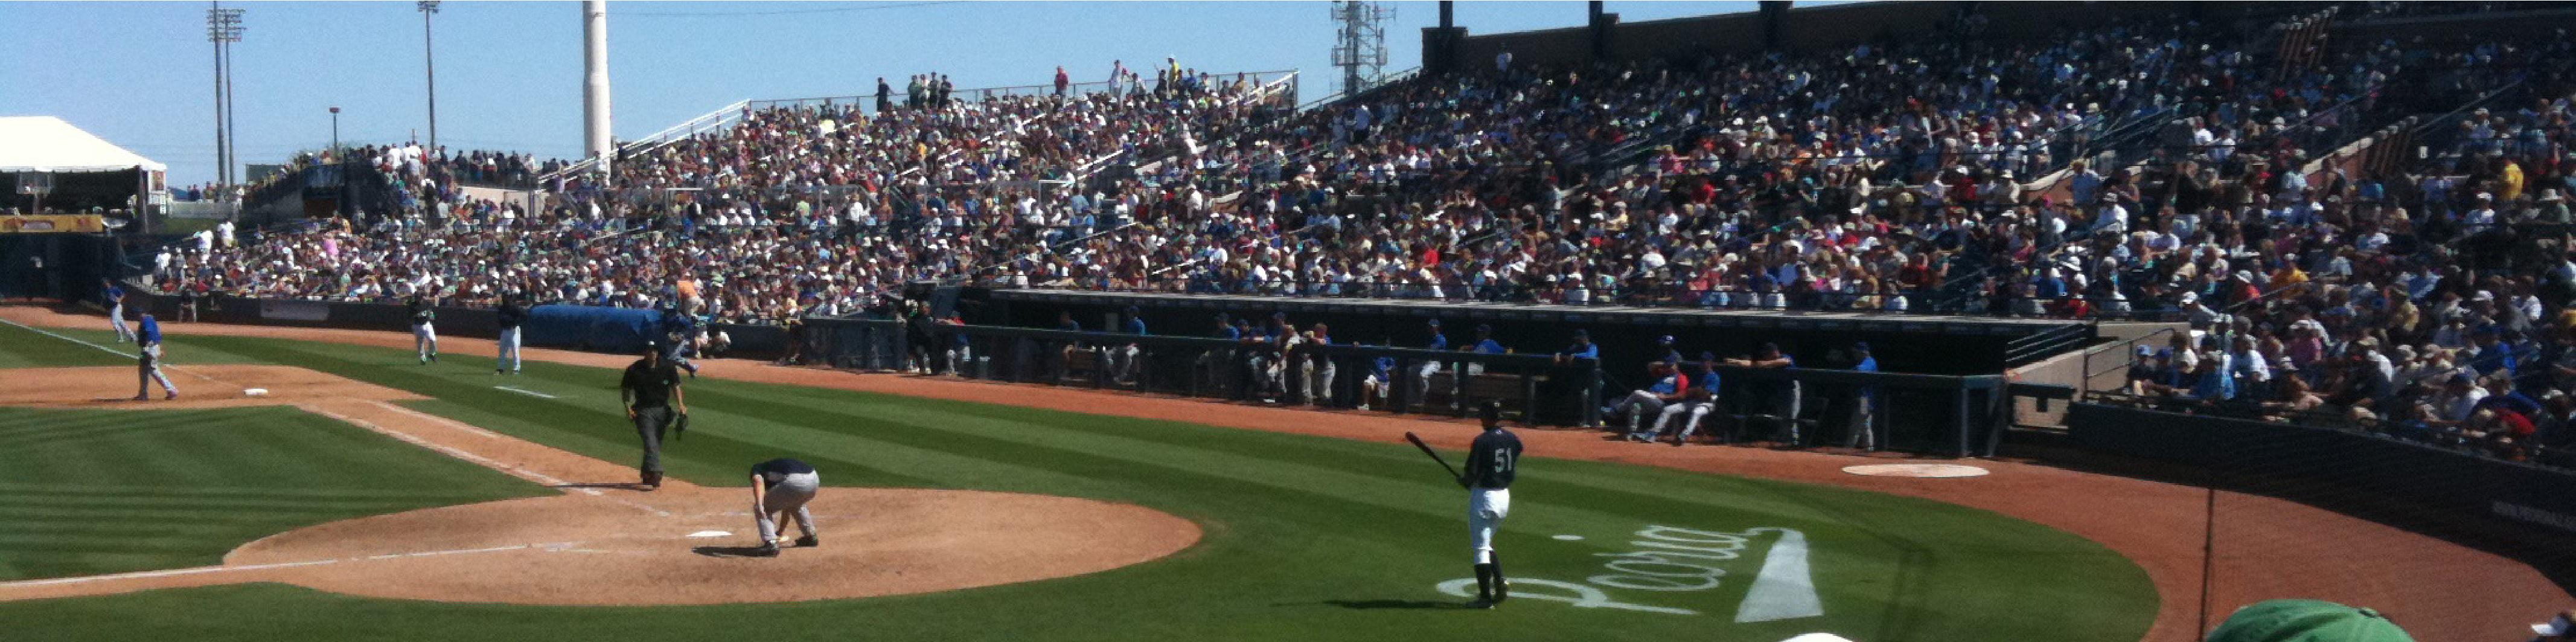
\includegraphics[width=\textwidth]{sampleteaser}
%   \caption{Seattle Mariners at Spring Training, 2010.}
%   \Description{Enjoying the baseball game from the third-base
%   seats. Ichiro Suzuki preparing to bat.}
%   \label{fig:teaser}
% \end{teaserfigure}

% \received{20 February 2007}
% \received[revised]{12 March 2009}
% \received[accepted]{5 June 2009}

%%
%% This command processes the author and affiliation and title
%% information and builds the first part of the formatted document.
\maketitle

\section{Introduction}
Fine-grained image recognition (FGIR) aims to distinguish between visually similar subcategories within a broader class. It is a challenging task due to small inter-class differences and large intra-class variations caused by pose, lighting, background changes. Although these categories are often organized hierarchically, early FGIR methods treat labels as flat categories \cite{zhang_part-based_2014, zheng_learning_2017}, ignoring semantic structure. This limits their ability to exploit hierarchical cues, resulting in suboptimal performance \cite{chen_fine-grained_2018}. 

Hierarchical FGIR addresses this by leveraging multi-level semantic relationships, using coarse-level predictions to guide fine-grained classification. Several approaches have explored this direction, such as granularity specific classifiers \cite{chang_your_2021} and hierarchically discriminative loss functions \cite{chen_fine-grained_2018}. However, these methods largely overlook a fundamental factor: the backbone itself. 

While backbone selection is known to influence standard FGIR \cite{ye_image_2024}, its role in hierarchical FGIR is underexplored. Most hierarchical FGIR methods continue to rely on a narrow set of backbones\cite{wang_multiple_2015, cerri_reduction_2016, chen_fine-grained_2018, chang_your_2021, chen_label_2022, chen_hierarchically_2024}, leaving open the question: \textbf{To what extent does the backbone influence performance in hierarchical FGIR?}

In this work, we conduct \textbf{the first study on backbone selection for hierarchical FGIR}. We benchmark a wide range of convolutional and transformer-based models across multiple datasets and hyperparameters, showing that backbone choice can yield drastically different outcomes, from state-of-the-art performance(91\% wAP on CUB for original ViT), to poor results (80\% wAP on CUB for CLIP), as observed in  Figure ~\ref{fig_four_plot}. To better capture both performance and robustness across evaluation runs, we introduce the \textbf{ADA ratio}. Using ADA, we are able to rank models by their peak performance and robustness across pretainings and hyperparameters.

Our study offers three main contributions: 
\begin{enumerate}
    \item We study 21 pretrained backbones (11 CNNs, 10 ViTs) in determining hierarchical FGIR performance. The right choice of backbone can \textbf{change wAP by up to 11\%}.
    \item We study the impact of hyperparameters across different models. The right choice of hyperparameter can \textbf{change wAP by up to 80\%}.
    \item Our analysis introduces the ADA ratio to assess both accuracy and robustness, offering a baseline for comparing and guidance for backbone selection in future hierarchical FGIR research.
    % \item Our analysis of 18 predictive highlights the challenge of predicting the performance hierarchical FGIR.
\end{enumerate}

\section{RELATED WORKS}
\subsection{Fine-Grained Image Recognition(FGIR)}
Early FGIR methods relied on part annotations or bounding boxes to guide localization \cite{zhang_part-based_2014}. While effective, these methods are difficult to scale due to the cost of annotations.  Later works leveraged image-level labels with attention mechanisms, such as MA-CNN \cite{zheng_learning_2017}, which learned part-aware features without extra supervision. However, these models ignored class hierarchies, limiting their ability to capture semantic structure and generalize across categories.

\subsection{Hierarchical Fine-Grained Image Recognition}
To address these limitations, hierarchical FGIR methods introduce multi-level prediction heads and hierarchy-aware losses. One of the first works, Multi-Granularity Descriptor (MGD) \cite{wang_multiple_2015}, used weakly supervised taxonomic descriptors. This was followed by methods like Hierarchical Semantic Embedding (HSE) \cite{chen_fine-grained_2018} and granularity-specific classifiers \cite{chang_your_2021}, which introduced hierarchy-aware loss functions and multi-level prediction heads.Though effective, these methods still struggle with class ambiguity within coarse groups and rely on a narrow set of backbone architectures.

\subsection{Backbone effect on FGIR}
Recent work has explored the impact of backbone architectures on transfer learning and FGIR. Kornblith et al. \cite{kornblith_better_2019} investigated whether ImageNet accuracy correlates with downstream performance on fine-grained tasks, concluding that it generalizes well. Nayman et al. \cite{nayman_diverse_2022} extended Kornblith et al.'s work by introducing alternative metrics to better predict transferability across tasks. However, both studies focus on general vision benchmarks and do not analyze hierarchical recognition explicitly, leaving open questions about how backbone design affects hierarchical FGIR.

\section{EXPERIMENT SETUP}
Our architecture follows the hierarchical pipeline of Chang et al. \cite{chang_your_2021}, where an image is processed by a shared feature encoder (backbone), followed by classifier heads for each taxonomy level. Each level targets labels from coarse to fine. We evaluated different backbones spanning two types, 10 Transformer (ViT-B) and 11 CNN (ResNet50). The 21 models are shown in Table \ref{tab:ada_ratio}.

Three datasets are used: \textbf{FGVC Aircraft} \cite{maji_fine-grained_2013}, \textbf{CUB-200-2011} \cite{wah_caltech-ucsd_2011}, and \textbf{Stanford Cars} \cite{krause_collecting_nodate}. Their hierarchies are constructed from Wikipedia class taxonomies following Chang et al. \cite{chang_your_2021}.

To assess model effectiveness in hierarchical FGIR, we measure several evaluation metrics measuring individual level, cross-level accuracy and robustness:
\begin{itemize}
    \item \textbf{Per-level accuracy}. The Top-1 classification accuracy of each level in the hierarchy. There are \textbf{3 hierarchical levels} at most, these are denoted by \textbf{L3, L2, L1, from coarsest to finest}.

    \item \textbf{Weighted Average Precision (wAP).}  
    to address class imbalance, wAP weights per-class accuracy by sample count
    wAP is defined as:
    \[
    wAP = \frac{1}{N} \sum_{k=1}^{K} n_k \cdot \text{Acc}_k
    \]
    where $K$ is the number of classes, $n_k$ is the number of samples in class $k$, $\text{Acc}_k$ is the accuracy for class $k$, and $N = \sum_{k=1}^{K} n_k$ is the total number of samples.
    
    \item \textbf{ADA ratio}. 
    inspired by the coefficient of variation \cite{brown_applied_1998}, this metric balances accuracy and robustness by measuring the ratio of standard deviation to mean accuracy across multiple runs.
    ADA ratio is defined as:
    \[
    ADA\ ratio = \frac{\sigma}{\mu} \times 100\% 
    \]
    where $\mu$ denotes the mean accuracy and $\sigma$ the standard deviation across evaluation runs. Specifically, on \cref{tab:ada_ratio} we computed the ADA ratio across different hyperparameters and datasets. Lower ADA ratio indicates a model achieves both high mean accuracy and low deviation, desirable characteristics in practical deployments. 
\end{itemize}

We compare 2 different training settings: fine-tuning (FT), where all parameters are updated, and frozen backbone (FZ), where only the classifier head is trained. All models are trained for 200 epochs with a batch size of 8. To study the impact of hyperparameters, we use two optimizers (SGD and AdamW) across 10 learning rates, SGD (0.3–0.003) with weight decay 0, and AdamW (0.005–0.000005) with weight decay 0.05. We employ cosine learning rate scheduler and mixed precision. During training we employ standard data augmentation (resize to 550×550, random crop to 448×448, horizontal flip). Center cropping is used during inference.

\begin{figure*}[!htb]
    \centering
    \begin{minipage}{0.41\linewidth}
        \centering
        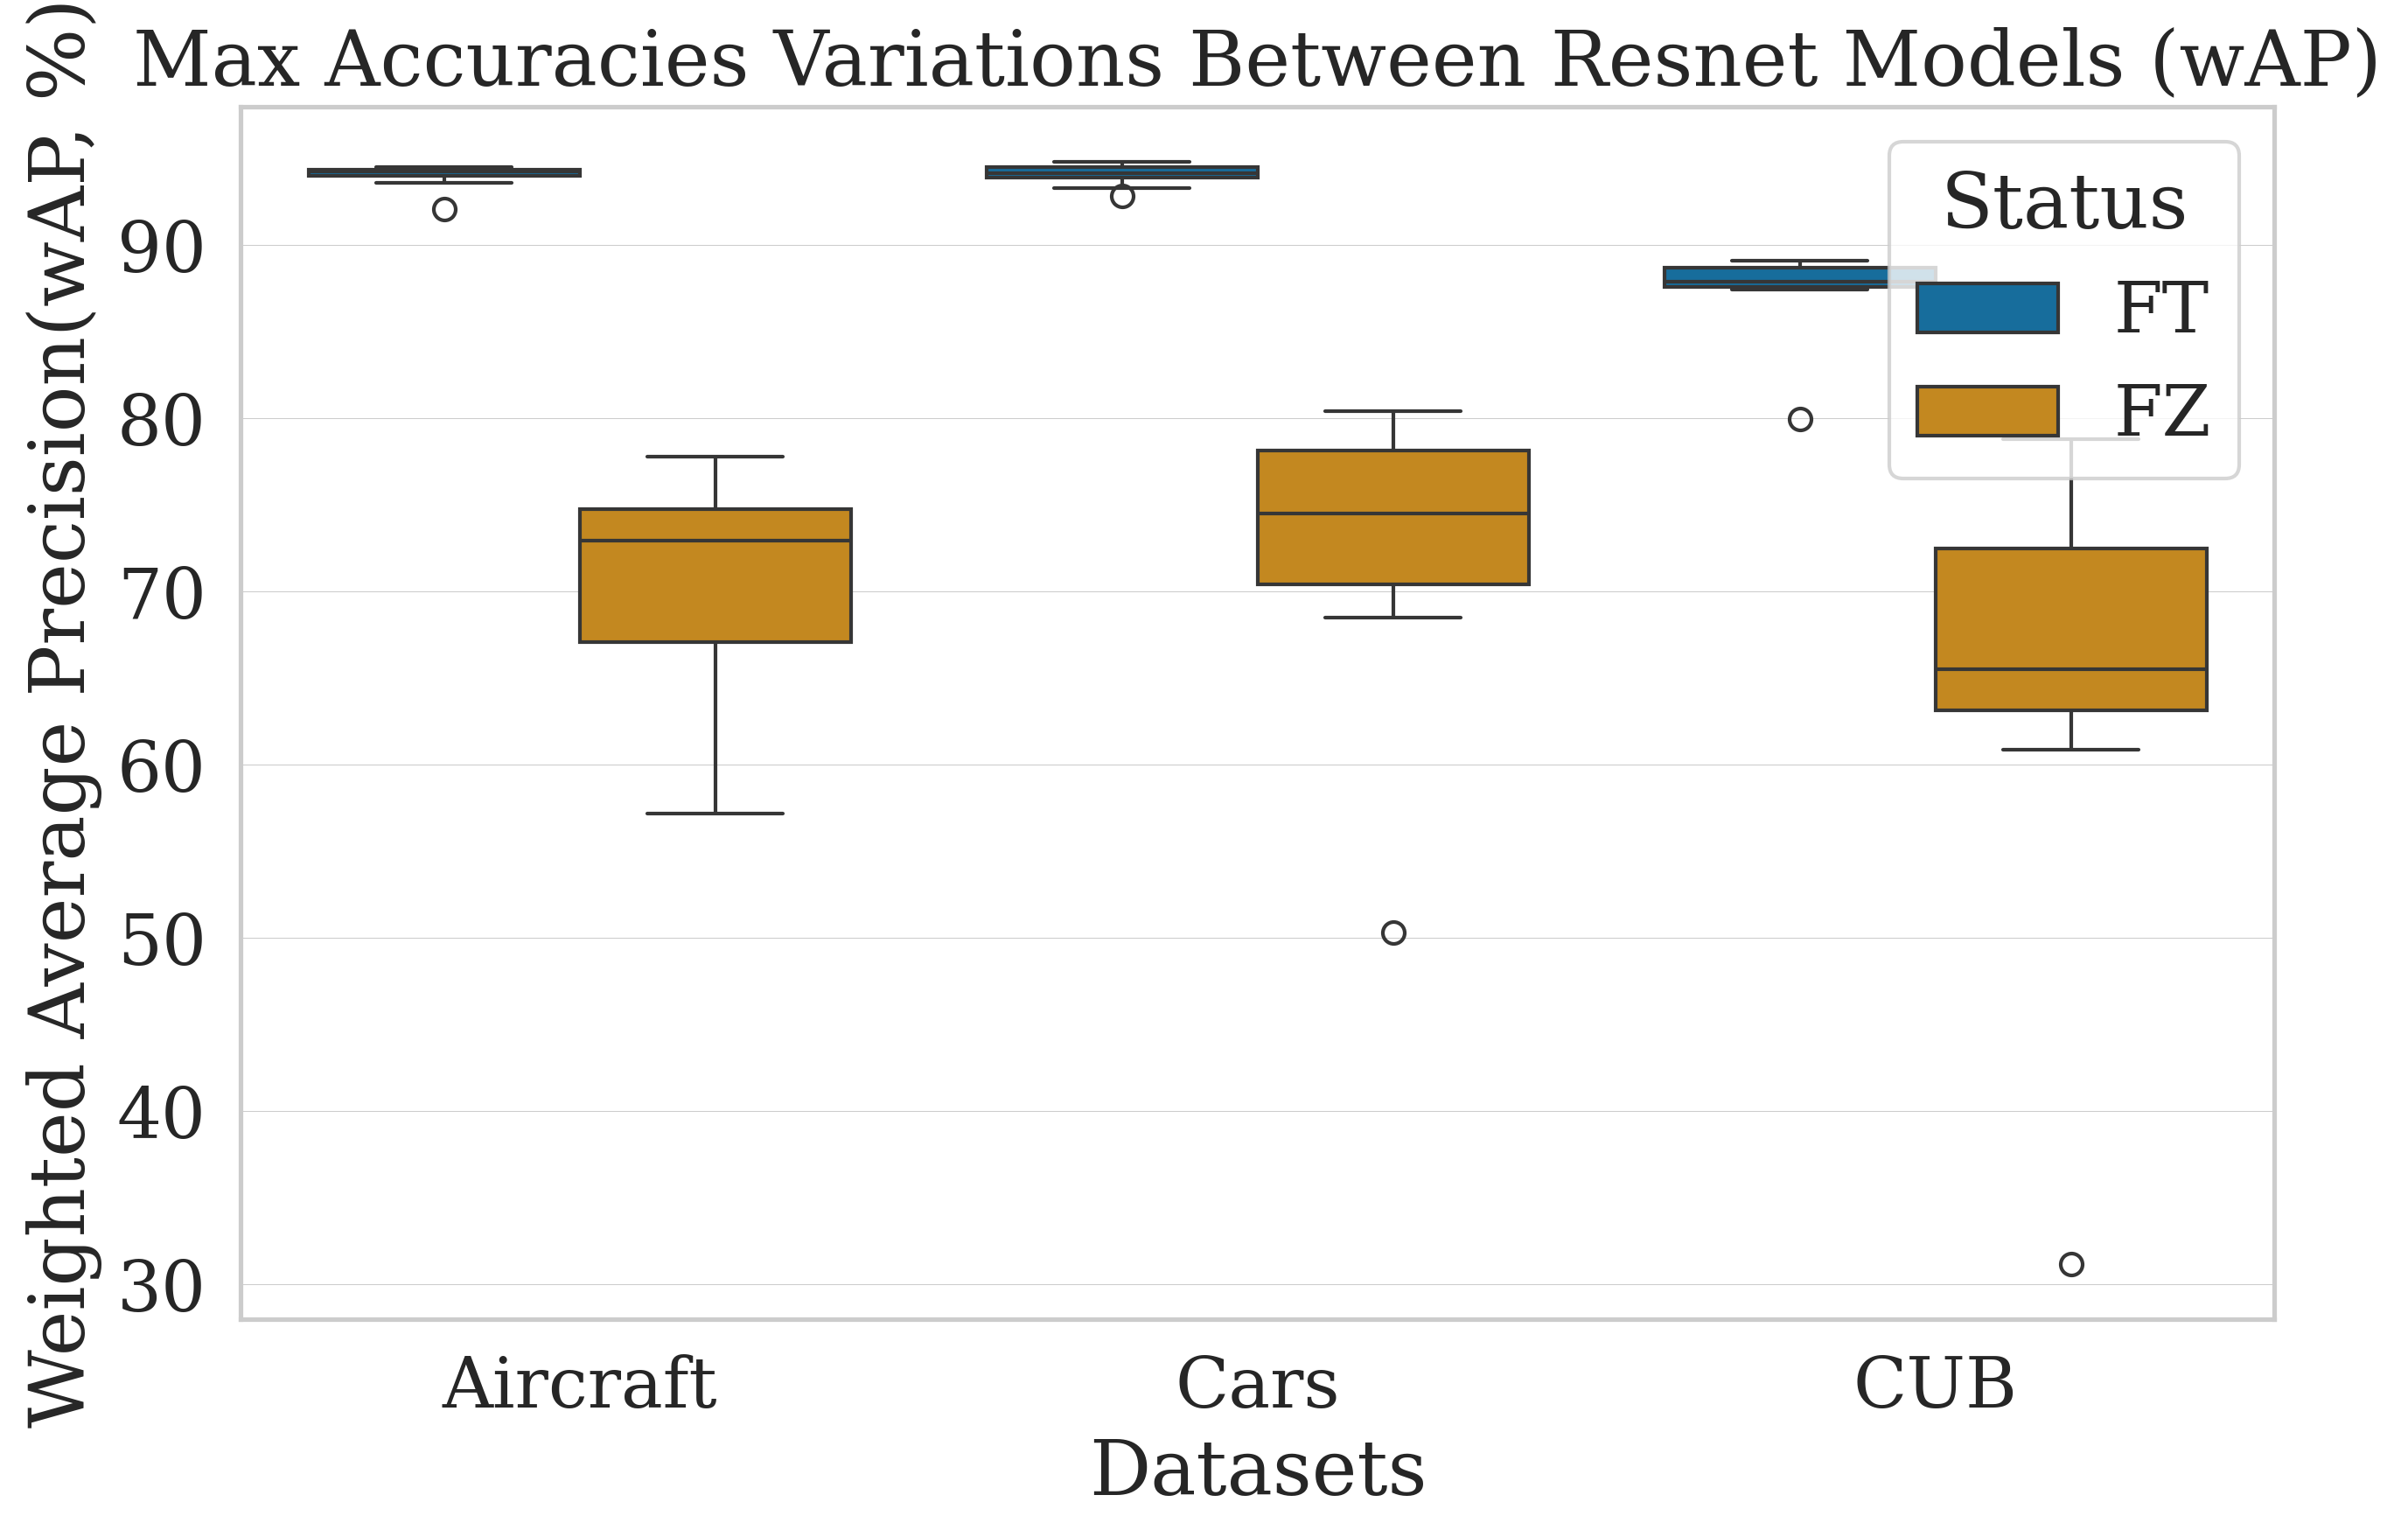
\includegraphics[width=\linewidth]{figures/imgs/performance_left.png}
        \label{fig_resnet_perf}
    \end{minipage}
    \hspace{0.01\linewidth} % Reduce spacing
    \begin{minipage}{0.40\linewidth}
        \centering
        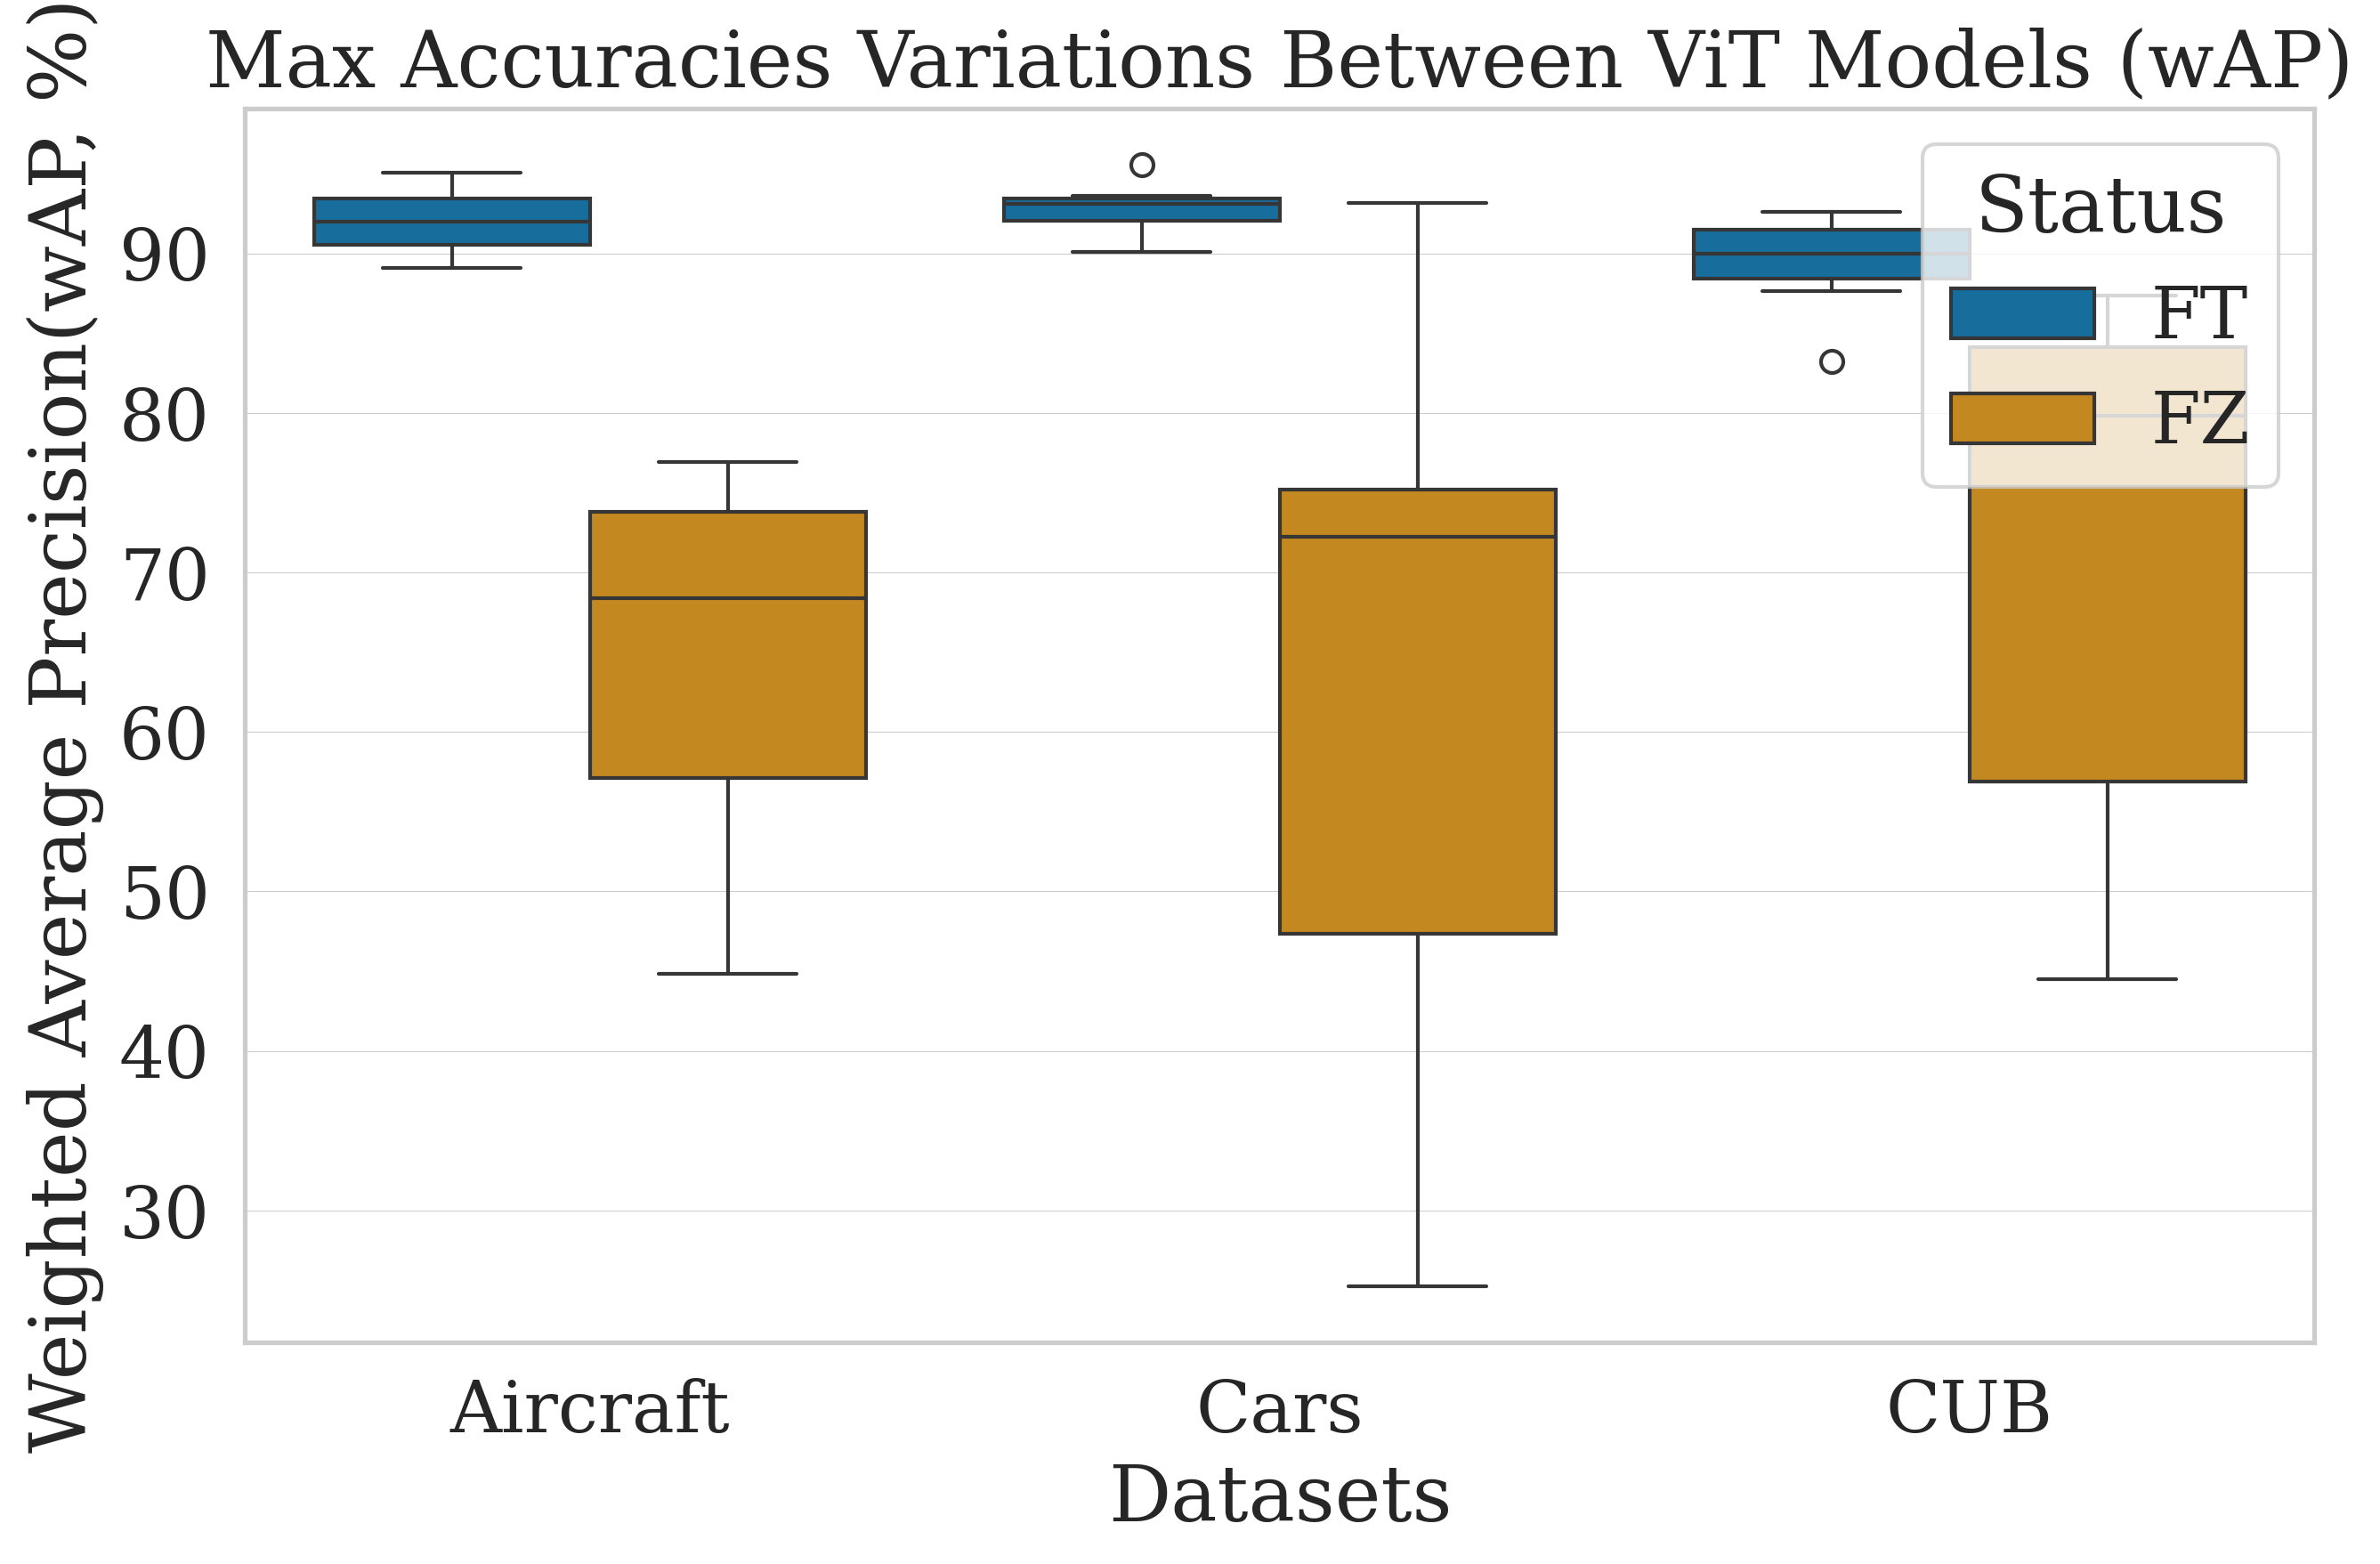
\includegraphics[width=\linewidth]{figures/imgs/performance_right.png}
        \label{fig_vit_perf}
    \end{minipage}
    \vspace{-0.55cm}
    \caption{Performance variability across backbone types and training modes. We compare fine-tuned (FT) and frozen (FZ) variants of ResNet (left) and ViT (right) models across hierarchical FGIR benchmarks.}
    \label{fig_performance}
\end{figure*}

\begin{table}[!htb]
    \centering
    \caption{ADA Ratio across different hyperparameters and datasets. Lower is better. Best and second best are \textbf{bold faced} and \underline{underlined}, respectively.}
    \label{tab:ada_ratio}
    \begin{tabularx}{\linewidth}{p{2.9cm}p{1.75cm}XX}
        \toprule
        Method & Fine-tuned & Frozen & Average \\
        \midrule
        \multicolumn{4}{>{\raggedright\arraybackslash}p{\linewidth}}{\textbf{ResNet50 models (CNN-based)}} \\
        \multicolumn{4}{>{\raggedright\arraybackslash}p{\linewidth}}{\textit{Fully-Supervised models}} \\
        RN TV1\cite{he_deep_2015} & 2.44 & 2.98 & 2.71 \\
        RN TV2\cite{he_deep_2015} & 1.39 & 1.24 & 1.31 \\
        RN Gluon\cite{he_bag_2018} & 2.61 & 1.41 & 2.01 \\
        RN IN21k-P\cite{ridnik_imagenet-21k_2021} & 1.54 & 1.04 & \underline{1.29} \\
        RN A1\cite{wightman_resnet_2021} & 2.42 & 0.96 & 1.69 \\
        \multicolumn{4}{>{\raggedright\arraybackslash}p{\linewidth}}{\textit{Semi-Supervised models}} \\
        RN IG1b\cite{yalniz_billion-scale_2019} & 4.28 & 1.18 & 2.73 \\
        RN YFCC100m\cite{yalniz_billion-scale_2019} & 3.53 & 1.5 & 2.51 \\
        \multicolumn{4}{>{\raggedright\arraybackslash}p{\linewidth}}{\textit{Self-Supervised models (Discriminative)}} \\
        RN SupCon\cite{khosla_supervised_2021} & 3.24 & 1.37 & 2.31 \\
        RN SwAV\cite{caron_unsupervised_2021} & \underline{1.33} & 1.46 & 1.39 \\
        RN MoCo v3\cite{chen_empirical_2021} & \textbf{1.18} & 1.32 & \textbf{1.25} \\
        \multicolumn{4}{>{\raggedright\arraybackslash}p{\linewidth}}{\textit{Self-Supervised models (Generative)}} \\
        RN SparK\cite{tian_designing_2023} & 5.67 & 3.92 & 4.8 \\
        \midrule
        \multicolumn{4}{>{\raggedright\arraybackslash}p{\linewidth}}{\textbf{ViT-B models (Transformer-based)}} \\
        \multicolumn{4}{>{\raggedright\arraybackslash}p{\linewidth}}{\textit{Fully-Supervised models}} \\
        ViT\cite{dosovitskiy_image_2021} & 11.35 & 1.01 & 6.18 \\
        DeiT\cite{touvron_training_2021} & 12.79 & 0.77 & 6.78 \\
        ViT IN21k-P\cite{ridnik_imagenet-21k_2021} & 17.43 & 1.98 & 9.7 \\
        DeiT 3 (IN1k)\cite{avidan_deit_2022} & 13.55 & 1.06 & 7.31 \\
        DeiT 3 (IN21k)\cite{avidan_deit_2022} & 18.42 & \textbf{0.59} & 9.51 \\
        \multicolumn{4}{>{\raggedright\arraybackslash}p{\linewidth}}{\textit{Self-Supervised models (Discriminative)}} \\
        ViT MoCo v3\cite{chen_empirical_2021} & 20.13 & 1.24 & 10.68 \\
        ViT DINO\cite{caron_emerging_2021} & 42.36 & 0.96 & 21.66 \\
        ViT CLIP\cite{cherti_reproducible_2023} & 52.52 & \underline{0.63} & 26.58 \\
        ViT SigLIP v2\cite{tschannen_siglip_2025} & 31.34 & 2.1 & 16.72 \\
        \multicolumn{4}{>{\raggedright\arraybackslash}p{\linewidth}}{\textit{Self-Supervised models (Generative)}} \\
        ViT MAE\cite{he_masked_2021} & 28.2 & 4.44 & 16.32 \\
        \bottomrule
    \end{tabularx}
\end{table}

\begin{figure}[ht]
    \centering
    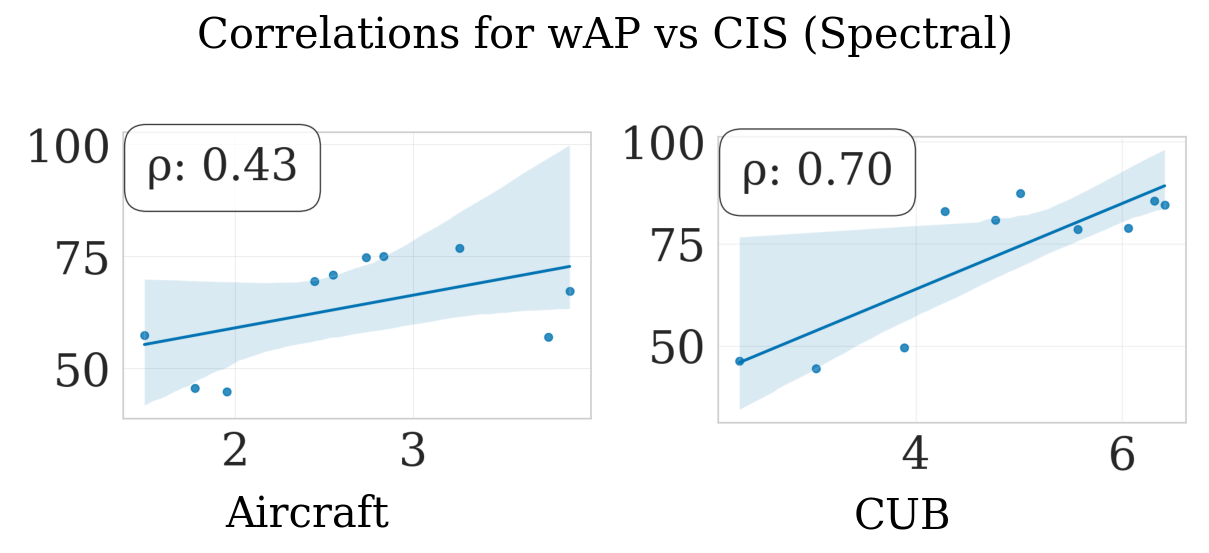
\includegraphics[width=0.9\linewidth]{figures/imgs/example_corr(1).png}
    \caption{Correlation plot between wAP vs. CIS(Spectral) for ViT models under frozen settings. Left side is correlation on Aircraft. Right side is correlation on CUB} 
    \label{fig_example_corr}
\end{figure}

\section{RESULTS}
\subsection{Impact of Backbone and Pretraining}
\subsubsection{Backbone Choice Drives Performance}
\cref{fig_performance} highlights how backbone selection alone can lead to vastly different outcomes. Among ResNets, MoCoV3 performs best (94\% wAP on Aircraft), while the worst performing one, Spark obtains 92\% wAP. ViT models show larger performance variance: SigLIP-v2 excels on Aircraft (94\%) and Cars (95\%), while original ViT excels CUB (91\%). In contrast, DINO performs worst with 87\% on Aircraft and 89\% on Cars. These findings shows that backbone selection, especially for ViTs, can lead to \textbf{state-of-the-art performance or degraded results}.

\begin{figure}[ht]
    \centering
    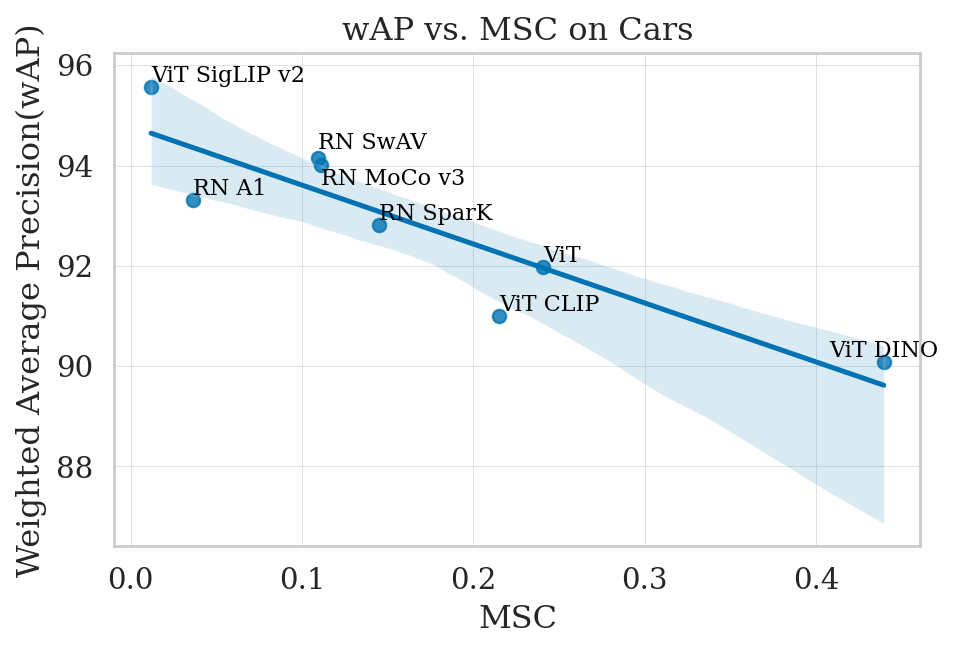
\includegraphics[width=0.85\linewidth]{figures/imgs/example_plot.png}
    \caption{Plot showing wAP vs. MSC for the Top-2 and Worst-2 Resnet and ViT fine-tuned models. ViT SigLiP is far away from the rest of the ViT.} 
    \label{fig_example_metric}
\end{figure}

\subsubsection{Resnet models do better on machines, but ViT models
do better on animals}
In Fig. \ref{fig_performance} and Fig. \ref{fig_four_plot} \textbf{ResNet models} generally \textbf{perform better} on \textbf{Aircraft and Cars}, while \textbf{ViTs do better} on \textbf{CUB}. This aligns with Ye et al.\cite{ye_image_2024}, which suggests that \textbf{objects with more dynamic shapes} (e.g. animals) \textbf{benefit} more from the \textbf{self-attention mechanism} in transformers. In contrast, \textbf{objects with more static shapes} (e.g. machines) \textbf{benefit} from the \textbf{inductive biases} in CNNs. Also, ImageNet contains a substantial number of bird-related images, which may have contributed to a performance boost for ViT models on the CUB dataset.

However, we observe \textbf{an exception}: \textbf{SigLIP}, a ViT model, achieves \textbf{better performance} on \textbf{Aircraft and Cars} than the \textbf{best ResNet model}, challenging this observation. To explain this, we employ \textbf{Mean Silhouette Coefficient (MSC)} \cite{rousseeuw_silhouettes_1987}, which quantifies the quality of feature clustering based on inter-class separation\cite{islam_broad_2021} and intra-class variance\cite{islam_broad_2021}. Higher values indicate well-separated and compact class clusters, while lower values imply more ambiguous features. We plot the Top-2 and Worst-2 wAP vs MSC for clarity, as observed in \cref{fig_example_metric}, SigLIP obtains lower MSC compared to other ViTs, suggesting tighter and less distinct feature representations. We also observed that ResNets obtains lower MSC than ViTs, while SigLiP obtains lower values than ResNets. This indicate that \textbf{performance stems from learned representations during pretraining rather than only architectural biases}.

To further understand the mechanisms behind effective backbone representations for hierarchical FGIR, we examine the predictive ability of various transferability metrics. This includes 7 metrics from prior work \cite{kornblith_better_2019, nayman_diverse_2022} including \textit{ImageNet1k Accuracy \cite{kornblith_better_2019}, CKA Average \cite{kornblith_why_2021}, MSC \cite{rousseeuw_silhouettes_1987}, Intra-Class Variance\cite{islam_broad_2021}, Inter-Class Separation\cite{islam_broad_2021}, CIS (Clustering)\cite{nayman_diverse_2022}, CIS (Spectral)\cite{nayman_diverse_2022}}, and 11 additional metrics including \textit{CKA First Layer, CKA Last Layer, CKA Low Layers, CKA Mid Layers, CKA High Layers, Normalized Distance, L2 Norm, CIS (CKA First Layer), CIS (CKA Last Layer), CIS (Distance First Layer), CIS (Distance Last Layer)}.  While some metrics showed high degree of correlation under certain datasets and settings, none of the metrics demonstrate consistent predictive performance for transferability; even for metrics with high degree of correlation on standard image classification tasks \cite{kornblith_better_2019, kornblith_why_2021, nayman_diverse_2022}. We visualize this in \cref{fig_example_corr}; it shows the correlation of wAP vs CIS (Spectral) \cite{nayman_diverse_2022} of ViT models under frozen settings. We can observe that the metric have stronger correlation on CUB but less on Aircraft. This observation is consistent with the other metrics, leading to the conclusion that no single metric can predict the overall transferability performance. These findings \textbf{shows the need for transferability metrics tailored to hierarchical recognition due to its unique challenges}.

\begin{figure*}[!htb]
    \centering
    \begin{minipage}{0.43\linewidth}
        \centering
        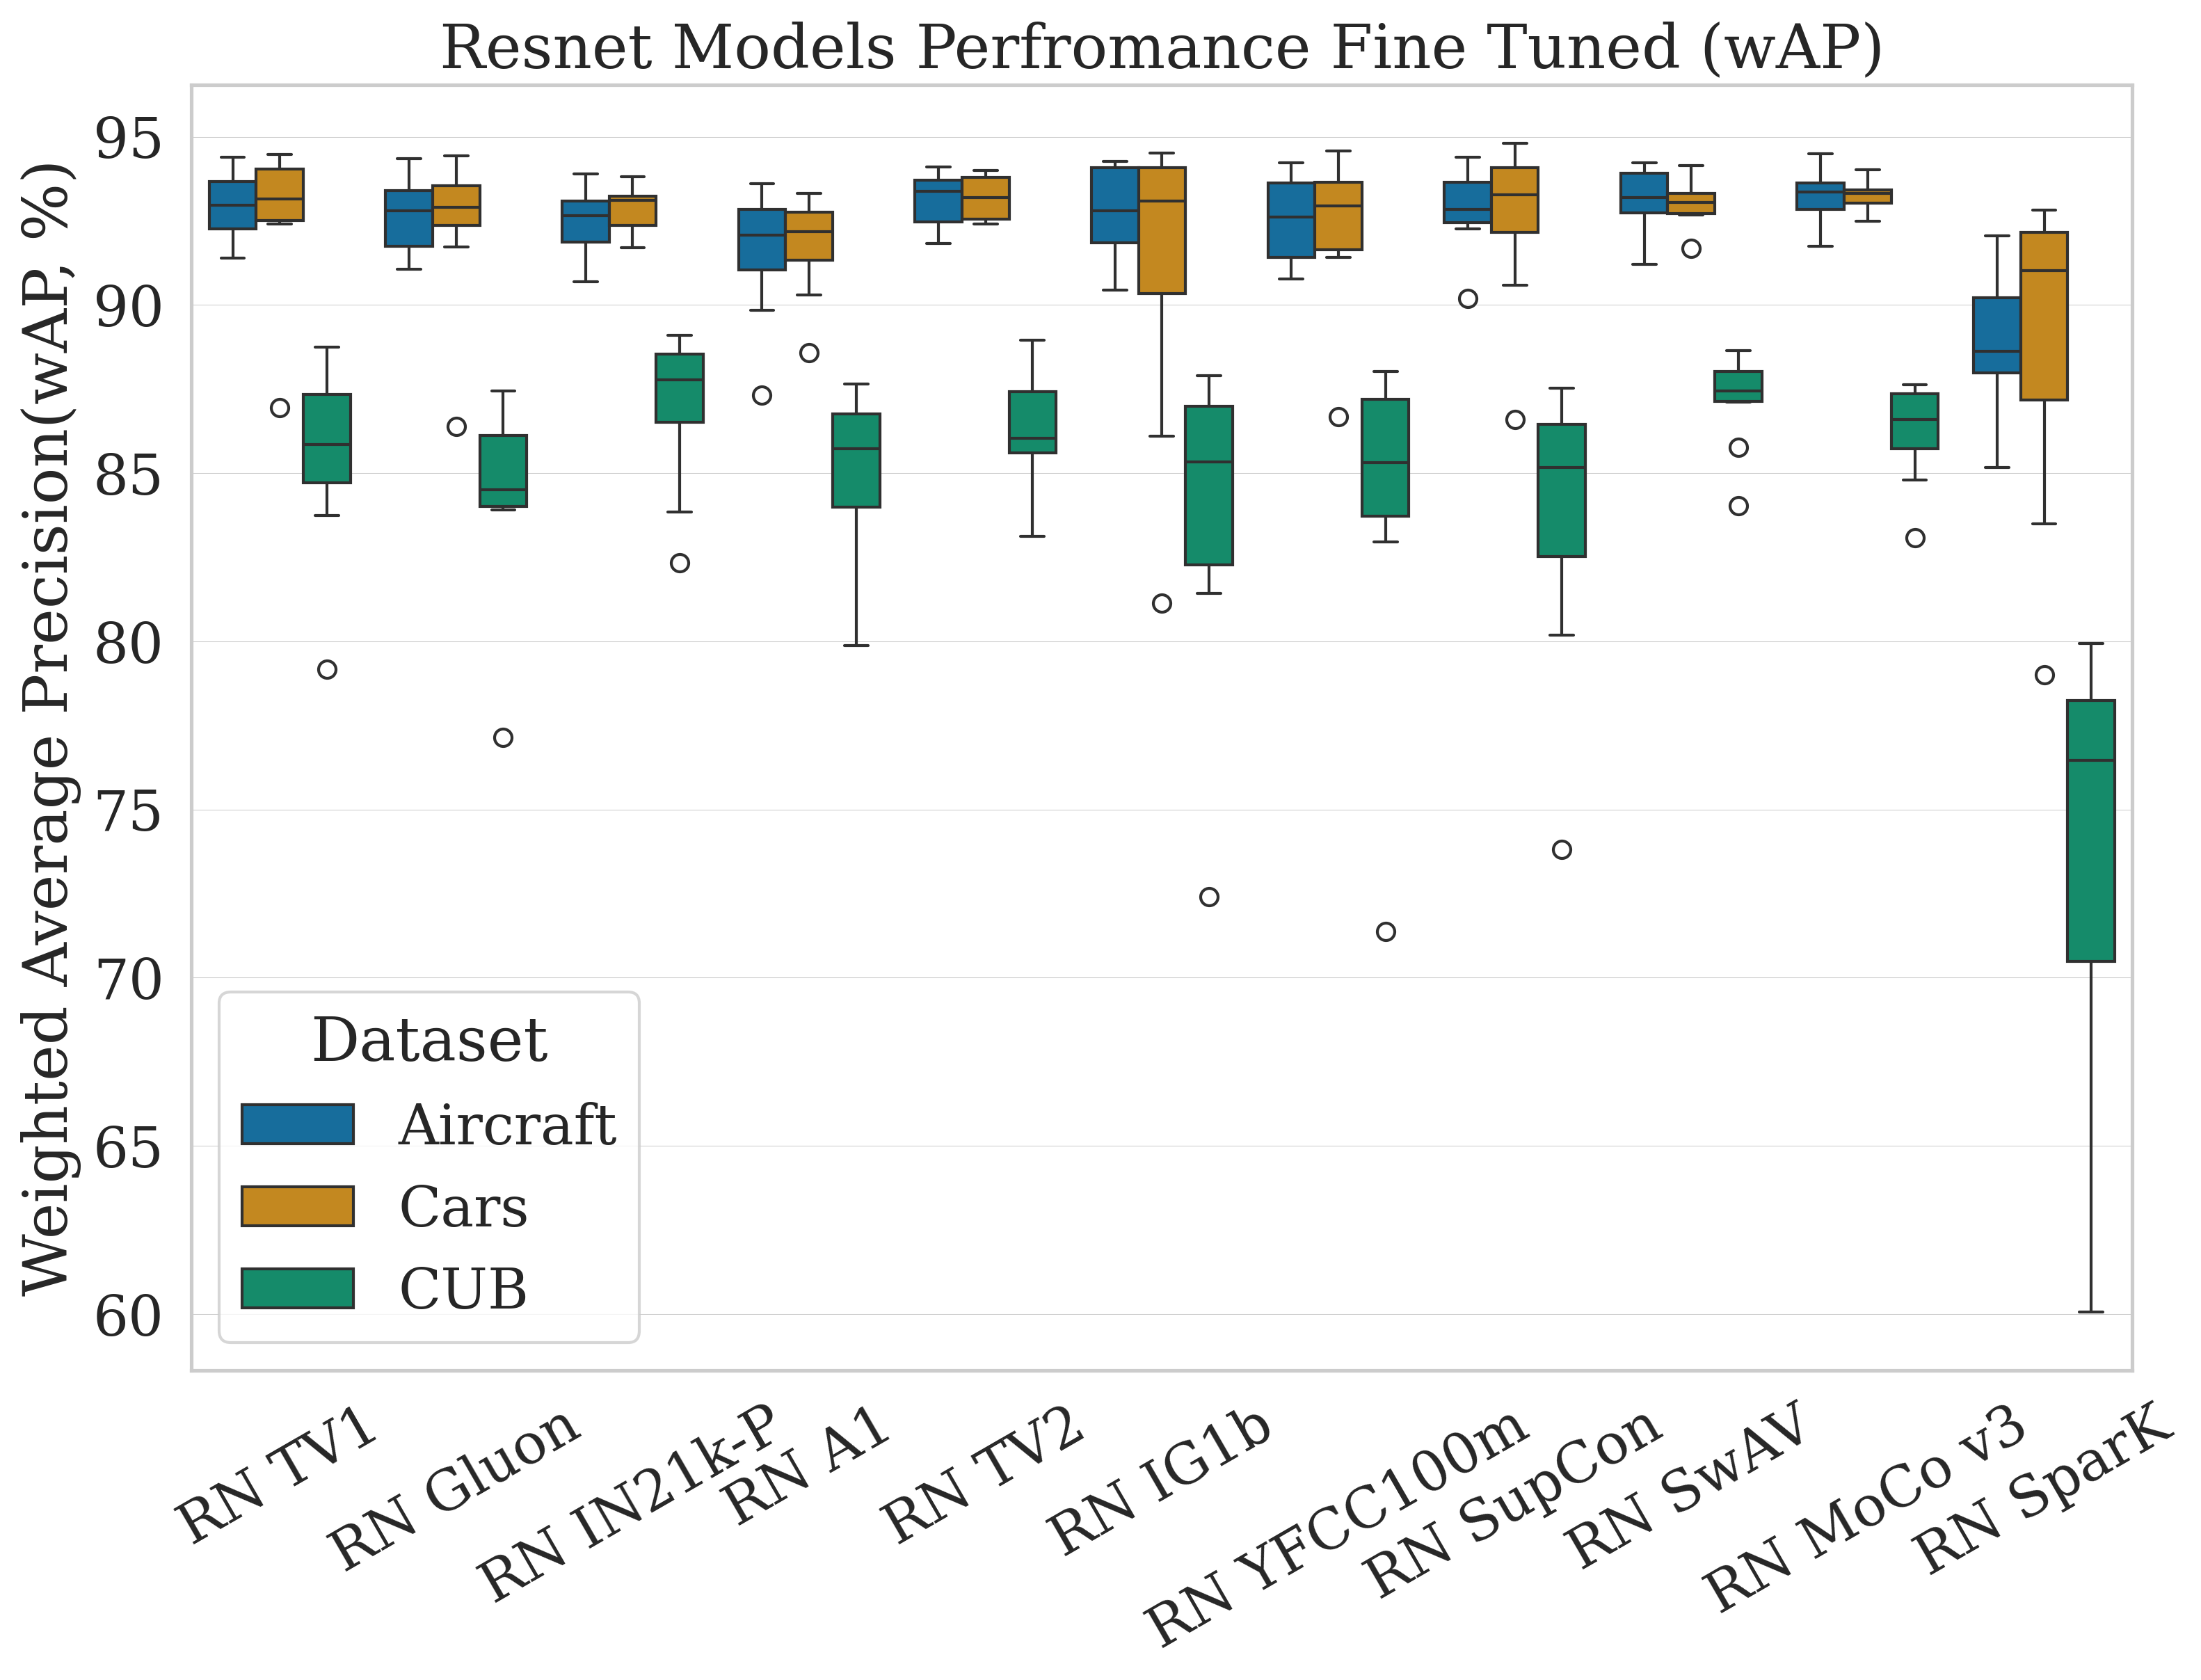
\includegraphics[width=\linewidth]{figures/imgs/rn_ft.png}
        \label{fig_rn_ft}
    \end{minipage}
    \hspace{0.01\linewidth} % Reduce spacing
    \begin{minipage}{0.43\linewidth}
        \centering
        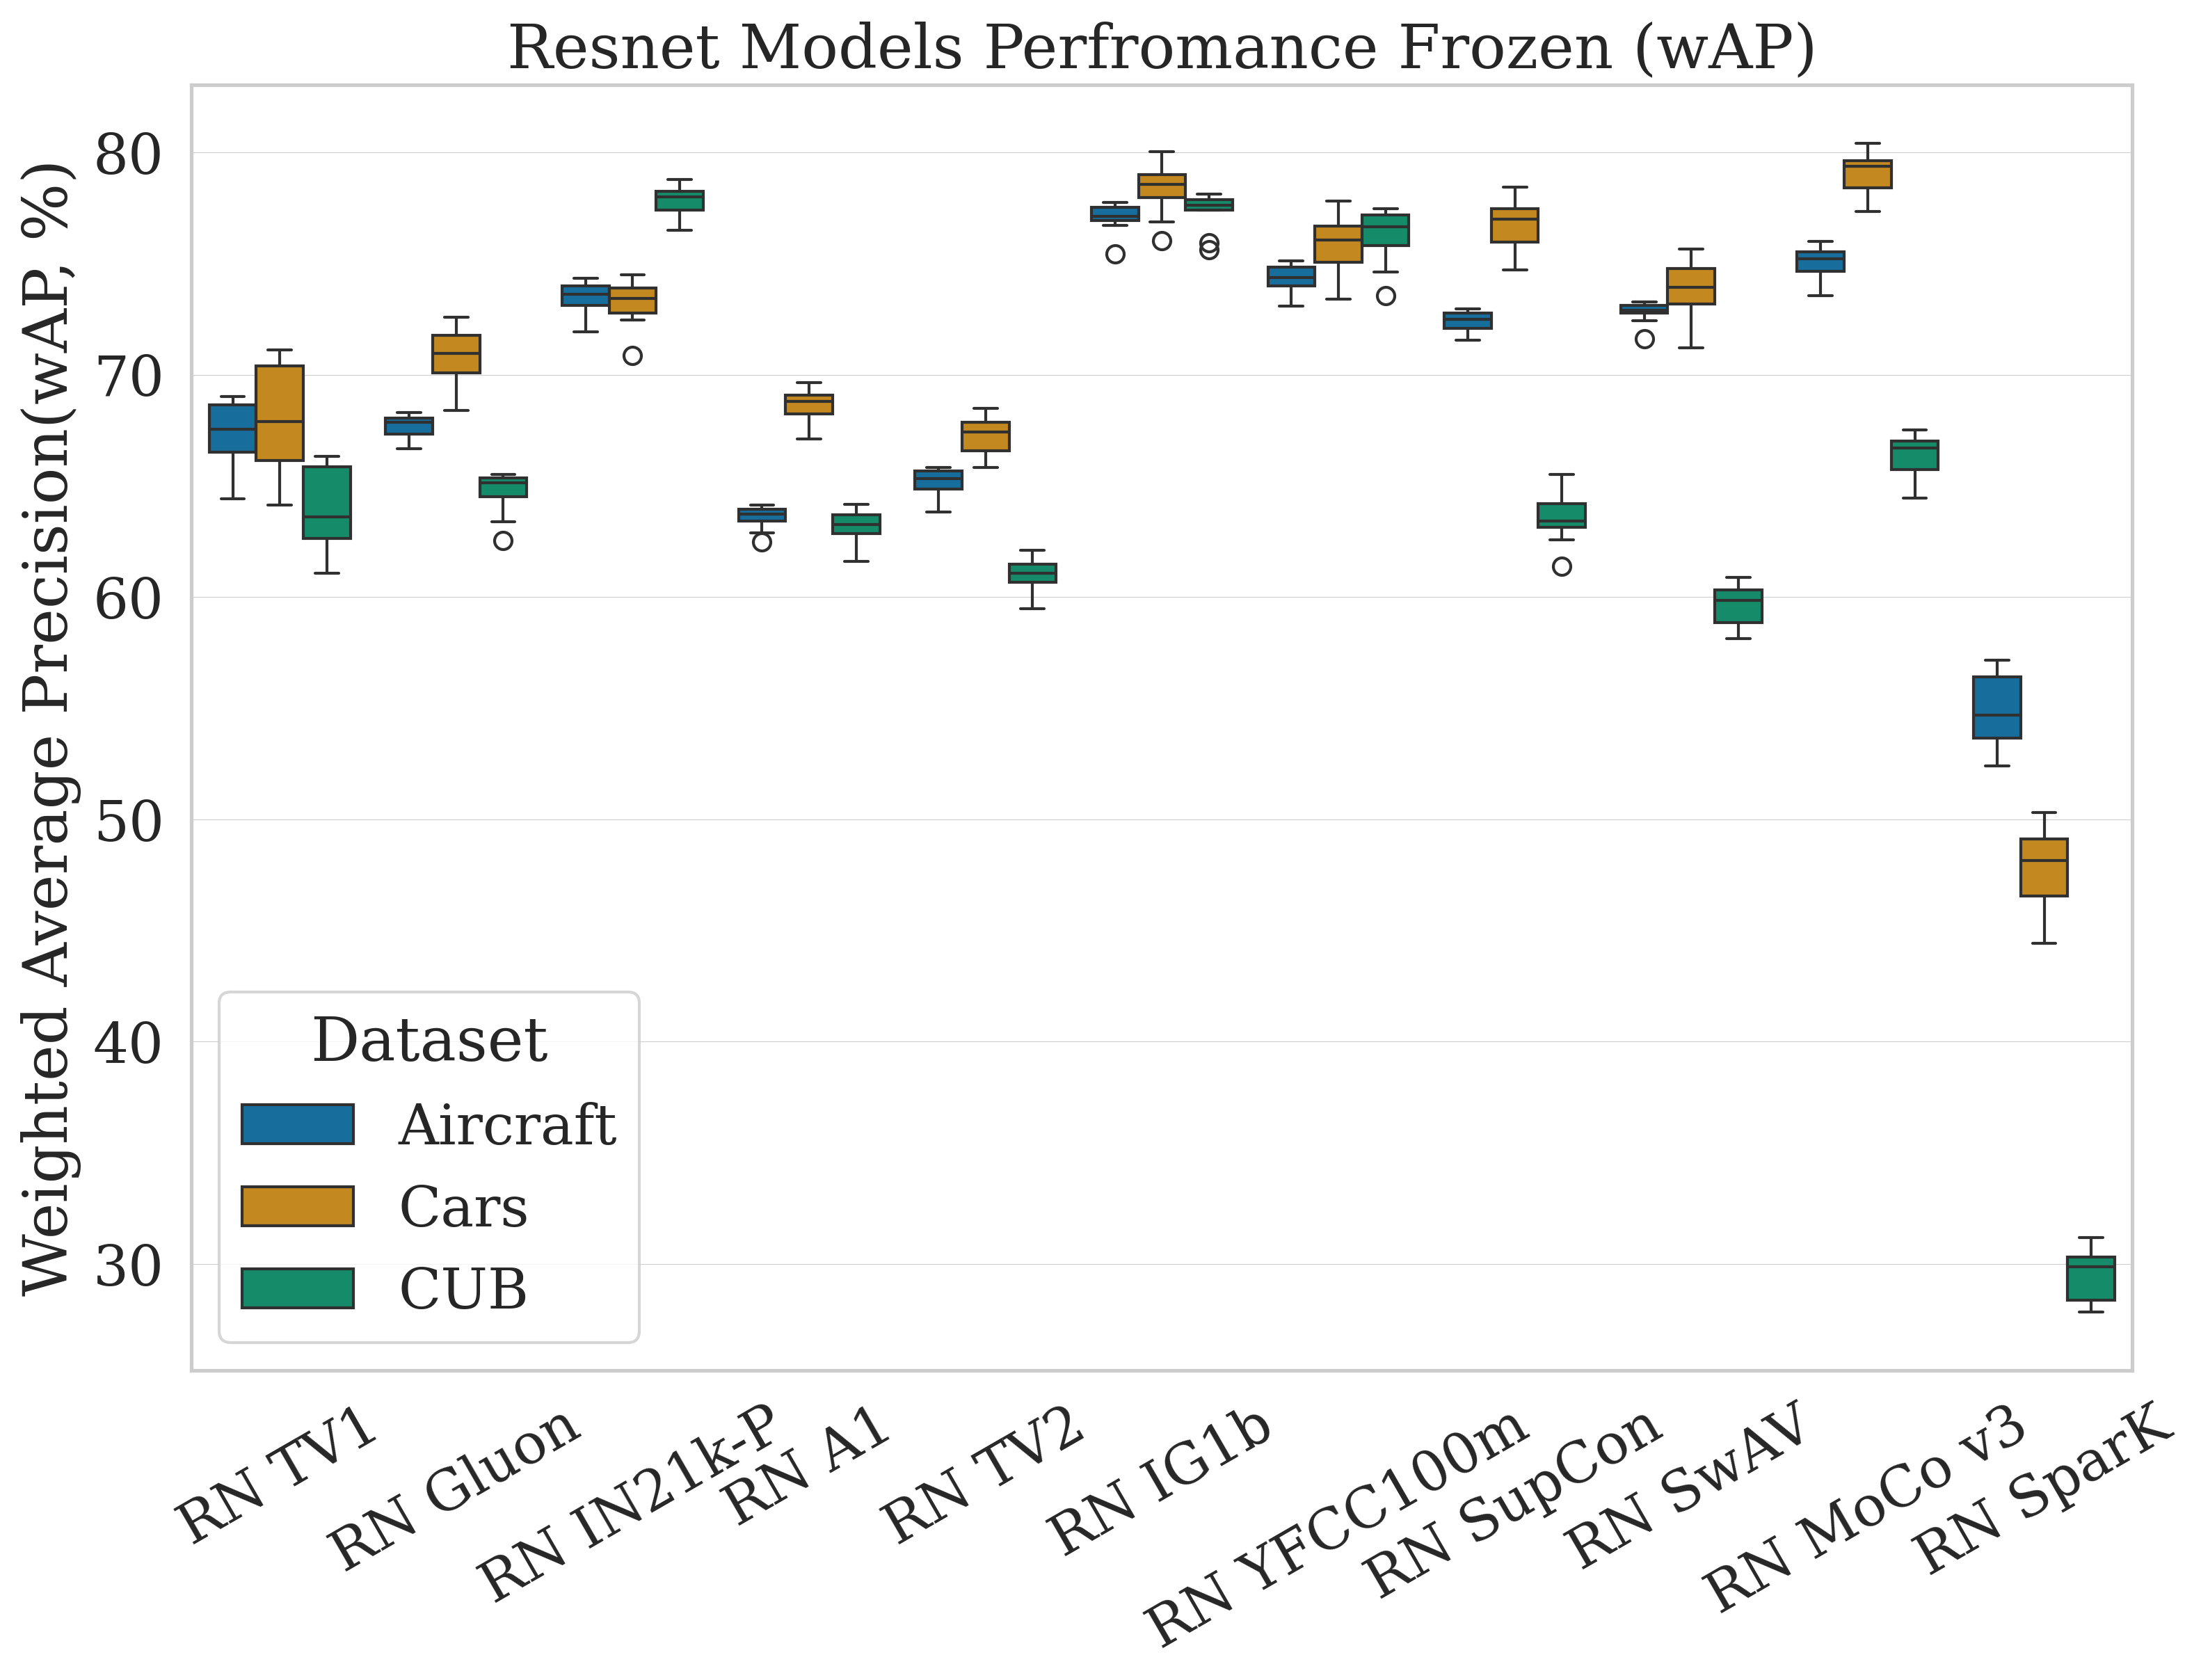
\includegraphics[width=\linewidth]{figures/imgs/rn_fz.png}
        \label{fig_rn_fz}
    \end{minipage}

    \centering
    \begin{minipage}{0.43\linewidth}
        \centering
        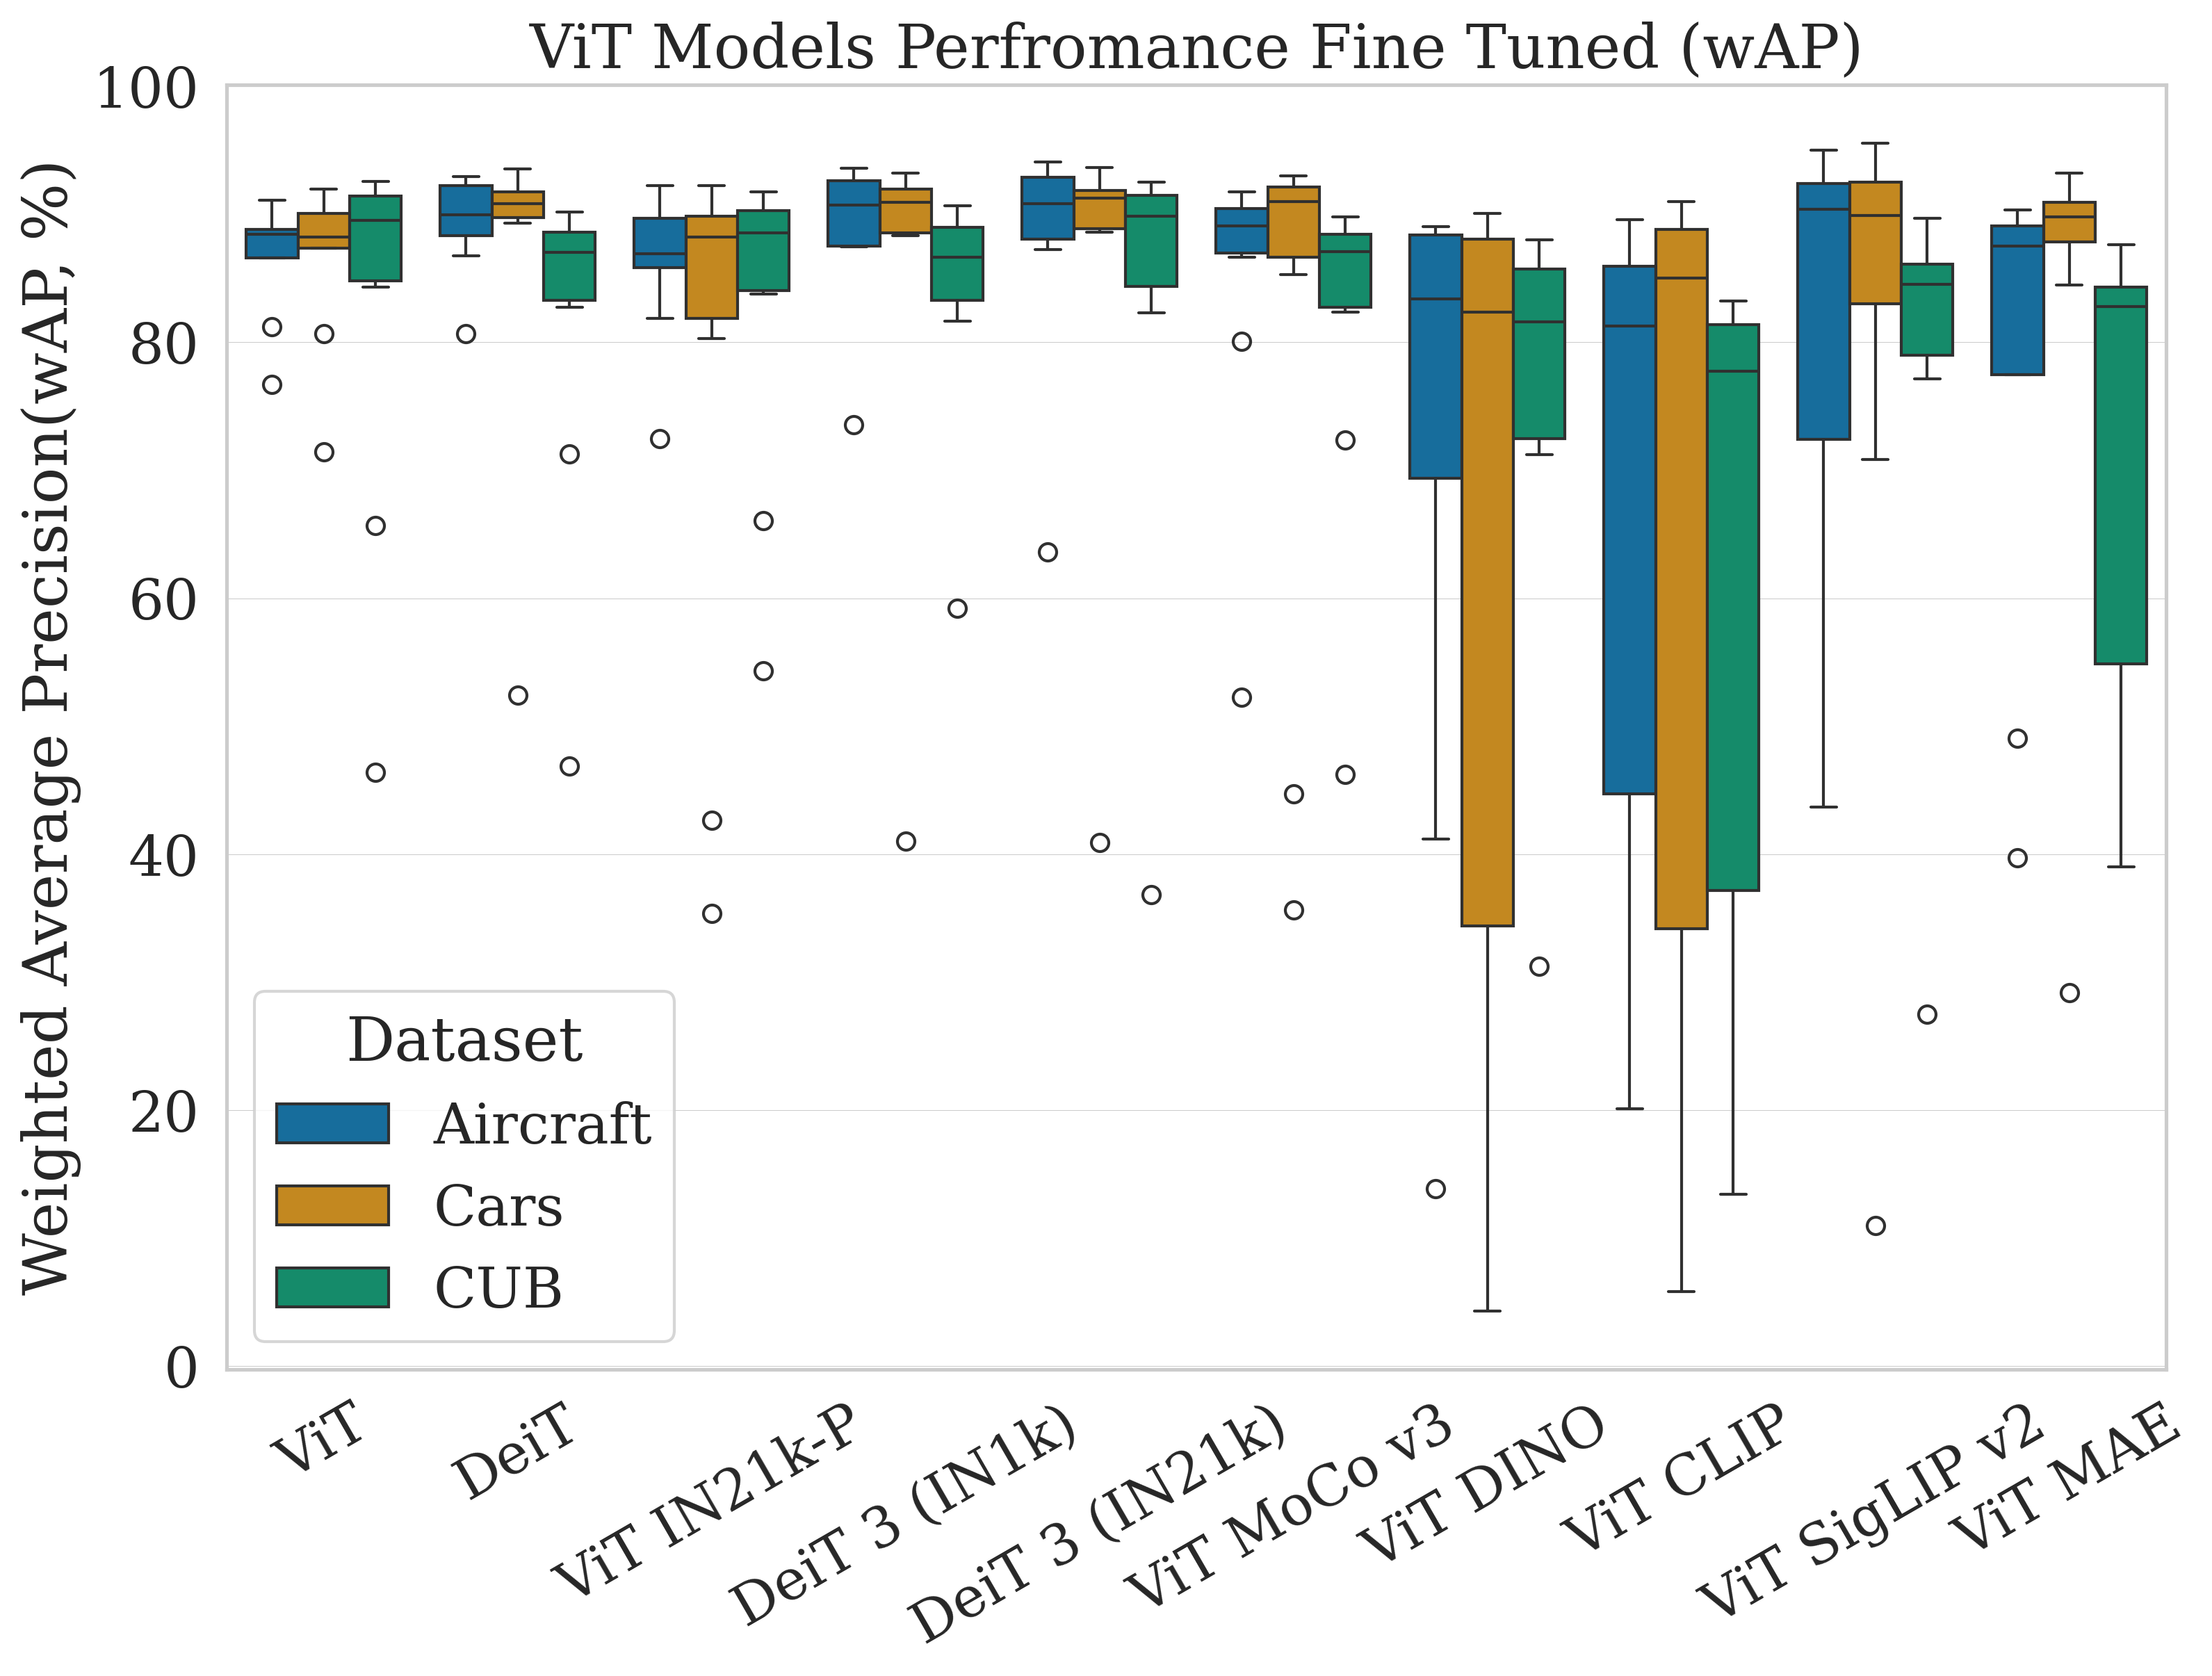
\includegraphics[width=\linewidth]{figures/imgs/vit_ft.png}
        \label{fig_vit_ft}
    \end{minipage}
    \hspace{0.01\linewidth} % Reduce spacing
    \begin{minipage}{0.43\linewidth}
        \centering
        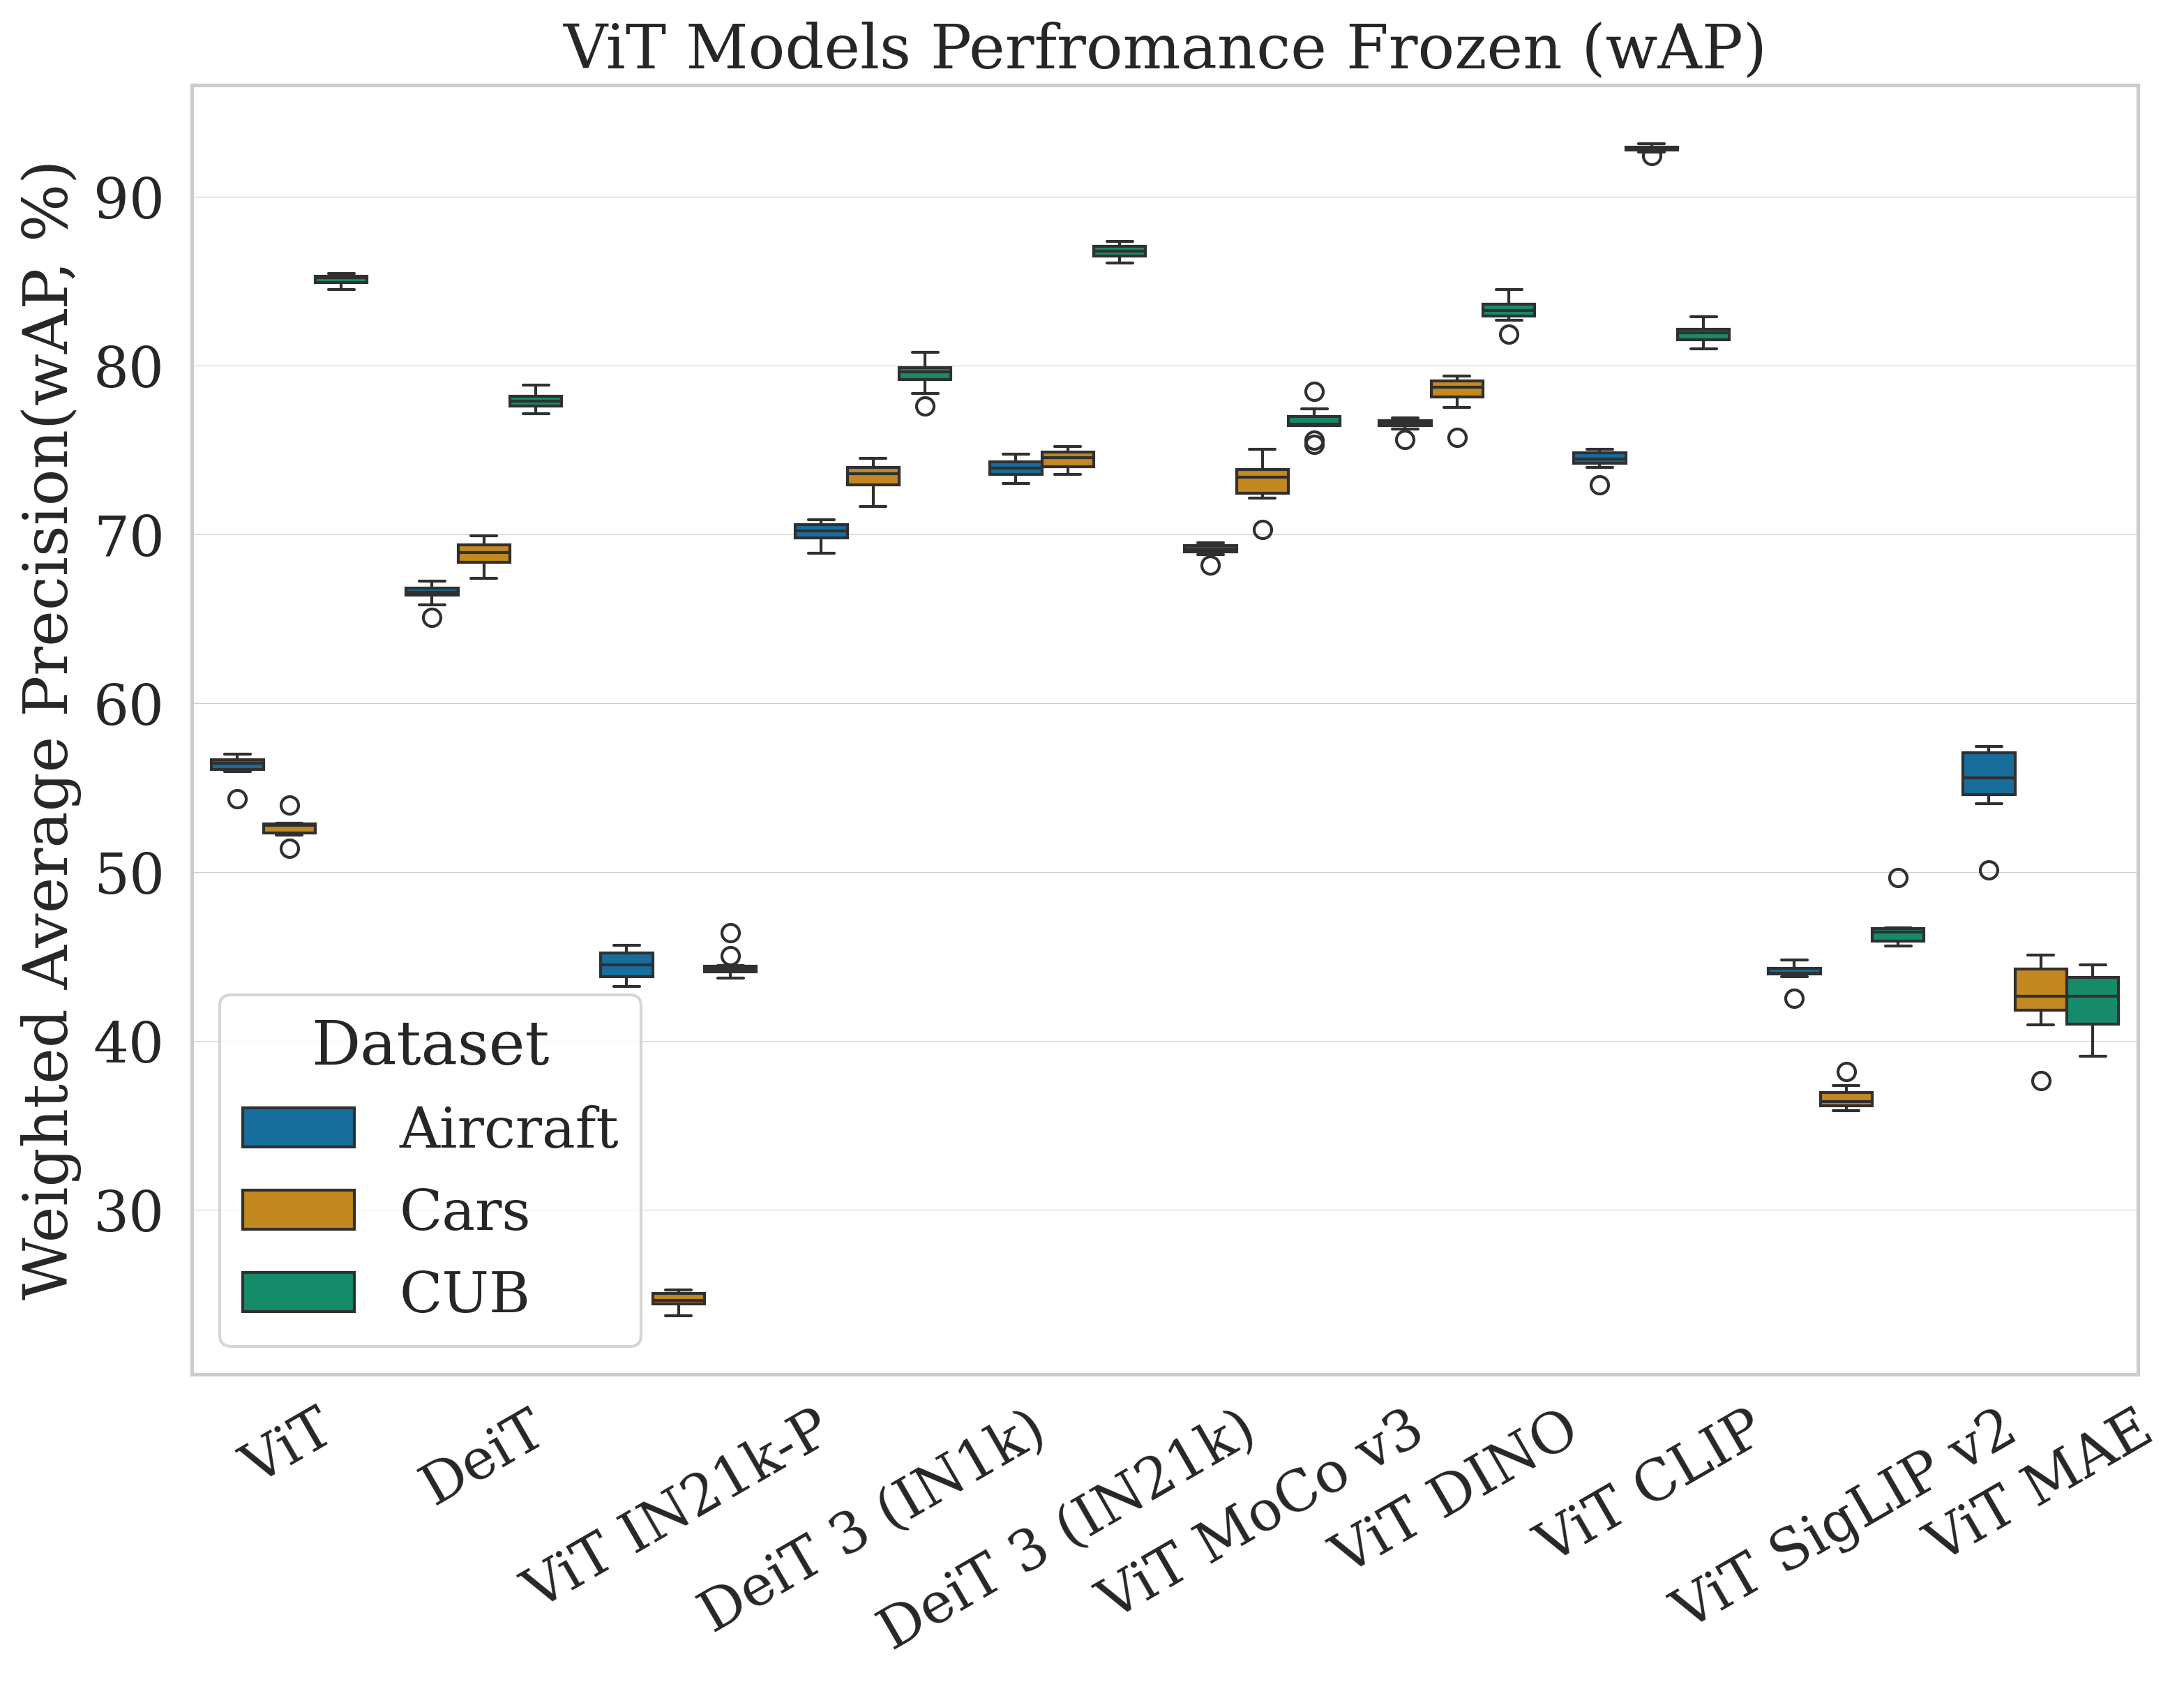
\includegraphics[width=\linewidth]{figures/imgs/vit_fz.png}
        \label{fig_vit_fz}
    \end{minipage}
    \vspace{-0.55cm}
    \caption{Backbone performance across training regimes. We compare ResNet (top) and ViT (bottom) models under fine-tuned (FT, left) and frozen (FZ, right) settings. Each plot shows the wAP performance distribution across models with different pretraining strategies.}
    \label{fig_four_plot}
\end{figure*}

\subsection{Impact of Hyperparameters}
\subsubsection{Resnet models are more robust than ViT models}
In Fig. \ref{fig_four_plot}, under \textbf{fine-tuned settings}, \textbf{ResNet models} pretrained with \textbf{discriminative objectives} (e.g., MoCoV3, SwAV) achieve the highest mean accuracy and lowest deviation. For \textbf{ViT models}, \textbf{fully supervised models} such as original ViT, DeiT, and DeiT3 also show strong fine-tuned performance with low deviation. In general, \textbf{ResNet models are more robust} than ViTs across pretraining and hyperparameter, as supported by consistently lower ADA ratios in Table \ref{tab:ada_ratio}. Among them, MoCoV3, a discriminative model, achieves the best ADA score across different settings. These results show discriminative ResNet models as a strong baseline for future hierarchical FGIR research.

\subsubsection{Scale of pretraining affects frozen performance}
In \ref{fig_four_plot}, under \textbf{frozen settings}, \textbf{Semi-Supervised models} (IG1b, YFCC300m) and the \textbf{IN21K-P model achieve the best results}.These 3 models are \textbf{pretrained on larger datasets, IG1b, YFCC300m, In21k accordingly}. For \textbf{ViT models}, \textbf{original ViT, DeiT (IN21K) and CLIP} models achieve high accuracy. They are also \textbf{pretrained} on \textbf{larger datasets}, \textbf{In21k, LAION5b accordingly}.

\subsubsection{Generative models underperform in frozen settings}
\textbf{Generative models} (e.g SparK, MAE) consistently \textbf{underperform in frozen settings} for both ResNet and ViT backbones, as observed in Fig. \ref{fig_four_plot}. Generative models, trained via masking and reconstruction objectives, appear to struggle with distinguishing fine-grained categories, indicating that \textbf{this strategy is not well suited for frozen settings in hierarchical FGIR tasks}.

\section{CONCLUSION}
The \textbf{choice of backbone} plays a \textbf{critical role} in hierarchical FGIR. By revisiting the pipeline of Chang et al. \cite{chang_your_2021} with \textbf{systematic backbone and hyperparameter selection}, we achieve \textbf{state-of-the-art results}, even with \textbf{older architectures}. Our findings further underscore that \textbf{hyperparameter tuning exerts a substantial influence} on model performance, with \textbf{ResNet models more robust than ViTs} regardless of hyperparameters. In particular, \textbf{discriminative models} (e.g., MoCoV3, SwAV) yield strong performance with both \textbf{high accuracy and low deviation}. The ADA ratio highlights the performance of models with hyperparameter choices in mind and offers a consistent basis for comparing architectures. As such, it serves as a useful metric for guiding model selection for future hierarchical FGIR research. We also evaluate 18 transferability metrics, but find that none consistently predict performance in the hierarchical FGIR setting. Our observation shows the need for new transferability metrics that account for the hierarchical structure of labels.

%%
%% The next two lines define the bibliography style to be used, and
%% the bibliography file.
\bibliographystyle{ACM-Reference-Format}
\bibliography{main}


\end{document}
\endinput
%%
%% End of file `sample-sigconf-authordraft.tex'.
